\documentclass[12pt]{article}

%%%%%% This thesis template was originally created by Zhiya Zuo and Erin Kaufman in May 2019, and revised by Marina Zhang and Erin Kaufman in July 2022. %%%%%%

%%%%%% start: define some names here %%%%%%
\newcommand{\longvertspacing}{~\\~\\~\\~\\~\\~\\}
\newcommand{\mylinespacing}{\vspace{1em}}
\newcommand{\myoptpg}{\textbf{THIS PAGE IS OPTIONAL}}
\newcommand{\mytitle}{Machine Learning Based Reconstruction Studies For DUNE Near Detector}
\newcommand{\sourcetitle}{Poul Anderson}
\newcommand{\myname}{Orgho Neogi}
%%%% replace My Degree with Doctor of Philosophy, Doctor of Musical Arts, Master of Science, Master of Arts, or Master of Fine Arts %%%%
\newcommand{\degreetype}{\capitalize{Doctor of Philosophy}} 
\newcommand{\mydegree}{\capitalize{Doctor of Philosophy}}
\newcommand{\myprogram}{\capitalize{Physics \& Astronomy}}
%%%% choose: May, August, December  %%%%
\newcommand{\mymonth}{May}
\newcommand{\myyear}{2024}
\newcommand{\myadvisor}{Jane Nachtman}
\newcommand{\committeememberA}{Yaser Onel}
\newcommand{\committeememberB}{Committee Member Name}
\newcommand{\committeememberC}{Committee Member Name}
\newcommand{\committeememberD}{Committee Member Name}
%%%%%% start: define some names here %%%%%%

\usepackage{geometry}
 \geometry{
 letterpaper,
 left=2.54cm,
 right=2.54cm,
 bottom=2.54cm,
 top=2.54cm,
 }
\usepackage[utf8]{inputenc}

%% ref related
\usepackage{varioref}
\usepackage[linktocpage=true]{hyperref}
\usepackage[capitalise,noabbrev]{cleveref}
%% toc
\usepackage{tocloft}
%%% dots: https://tex.stackexchange.com/questions/53898/how-to-get-lines-with-dots-in-the-table-of-contents-for-sections
\renewcommand{\cftsecleader}{\cftdotfill{\cftdotsep}}
\renewcommand{\cftfigleader}{\cftdotfill{\cftdotsep}}
\renewcommand{\cfttableader}{\cftdotfill{\cftdotsep}}
%%% adjust sectional unit title fonts in toc
\renewcommand{\cftsecfont}{\normalfont\MakeUppercase} 
\renewcommand{\cftsubsecfont}{\normalfont}
\renewcommand{\cftsubsubsecfont}{\normalfont}
\renewcommand{\cftsecpagefont}{\normalfont}
%%% use figure/table.num for the lot and lof
%\renewcommand{\cftfigfont}{Figure~\alph{fig}.}
%% source: https://tex.stackexchange.com/questions/419103/how-to-change-the-numbering-style-in-list-of-table-and-list-of-figures
\renewcommand{\cftfigpresnum}{Figure }
\renewcommand{\cftfigaftersnum}{.\hspace{1ex}}
\renewcommand{\cfttabpresnum}{Table }
\renewcommand{\cfttabaftersnum}{.\hspace{1ex}}
%%% increase spacing between entries in toc
\setlength{\cftparskip}{2ex}
%%% decrease spacing between number and title as well as indent
%\setlength{\cftfignumwidth}{10ex}
%\setlength{\cfttabnumwidth}{8ex}
\setlength{\cftfignumwidth}{10.5ex}
\setlength{\cfttabnumwidth}{8ex}
\setlength{\cftfigindent}{0ex}
\setlength{\cfttabindent}{0ex}
%%% title names
%%% center uppercase toc titles
%% https://tex.stackexchange.com/a/255699/154200
\renewcommand{\cfttoctitlefont}{\hspace*{\fill}\normalsize\MakeUppercase}
\renewcommand{\cftaftertoctitle}{\hspace*{\fill}}
\renewcommand{\contentsname}{table of contents}
\renewcommand{\cftlottitlefont}{\hfill\normalsize\MakeUppercase}
\renewcommand{\cftafterlottitle}{\hfill}
\renewcommand{\cftloftitlefont}{\hfill\normalsize\MakeUppercase}
\renewcommand{\cftafterloftitle}{\hfill}
%% this package binds all indices to toc
\usepackage[nottoc]{tocbibind}
%%% remove toc numbering
\makeatletter
\let\latexl@section\l@section
\def\l@section#1#2{\begingroup\let\numberline\@gobble\latexl@section{#1}{#2}\endgroup}
\let\latexl@subsection\l@subsection
\def\l@subsection#1#2{\begingroup\let\numberline\@gobble\latexl@subsection{#1}{#2}\endgroup}
\let\latexl@subsubsection\l@subsubsection
\def\l@subsubsection#1#2{\begingroup\let\numberline\@gobble\latexl@subsubsection{#1}{#2}\endgroup}
\makeatother
%% set figure path
\usepackage{graphicx}
\graphicspath{{figures/}}
%% captions
\usepackage{boxhandler}
\usepackage{caption}
\captionsetup{labelsep=period, justification=raggedright, singlelinecheck=false}
%% appendix
\usepackage{appendix}
%% biblatex
%\usepackage[style=apa,language=american,maxnames=4,minnames=3,sortcites=true]{biblatex}
%\DeclareLanguageMapping{american}{american-apa}
%\addbibresource{ref.bib}
%% uses times font
\usepackage{mathptmx}
%% set fontsize
\fontsize{12}{1} \selectfont
%% set line spacing
\usepackage{setspace}
\singlespacing
%% set par indent
%\usepackage{indentfirst}
\setlength{\parindent}{6.5ex}
%% customize heading styles
\usepackage[indentafter]{titlesec}
\usepackage[numbers]{natbib}
%%%% heading 1
\titleformat{\section}
  {\normalsize\center}
  {}
  {0pt}
  {\MakeUppercase}
%%%% heading 2
\titleformat{\subsection}
  {\normalsize\center\bf}
  {}
  {0pt}
  {\capitalize}
%%%% heading 3
\titleformat{\subsubsection}
  {\normalsize\bf}
  {}
  {0pt}
  {\capitalize}
%%%% heading 4
\titleformat{\paragraph}
  {\normalsize\bf\itshape}
  {}
  {0pt}
  {\capitalize}
%\titleformat{⟨command⟩}[⟨shape⟩]{⟨format⟩}{⟨label⟩}{⟨sep⟩}{⟨before-code⟩}[⟨after-code⟩]

%% a new center environment
\newenvironment{tightcenter}{%
  \setlength\topsep{0pt}
  \setlength\parskip{0pt}
  \begin{center}
}{%
  \end{center}
}
%% adjust quotation environment margin
\renewenvironment{quote}{%
   \list{}{%
     \leftmargin0cm   % this is the adjusting screw
     \rightmargin\leftmargin
   }
   \item\relax
}
{\endlist}

%%%%%% capitalize from stackexchange %%%%%% 
\usepackage{ifxetex}

\usepackage{xparse}

\ExplSyntaxOn
\NewDocumentCommand{\capitalize}{>{\SplitList{~}}m}
 {
  \seq_clear:N \l_capitalize_words_seq
  \ProcessList{#1}{\CapitalizeFirst}
  \seq_use:Nn \l_capitalize_words_seq { ~ }
 }
\NewDocumentCommand{\CapitalizeFirst}{m}
 {
  \capitalize_word:n { #1 }
 }

\sys_if_engine_pdftex:TF
 {
  \cs_set_eq:Nc \capitalize_tl_set:Nn { protected@edef }
 }
 {
  \cs_set_eq:NN \capitalize_tl_set:Nn \tl_set:Nn
 }

\cs_new_protected:Nn \capitalize_word:n
 {
  \capitalize_tl_set:Nn \l_capitalize_word_tl { #1 }
  \seq_if_in:NfTF \g_capitalize_exceptions_seq { \tl_to_str:n { #1 } }
   % exception word
   { \seq_put_right:Nn \l_capitalize_words_seq { #1 } } % exception word
   % to be uppercased
   { \seq_put_right:Nx \l_capitalize_words_seq { \tl_mixed_case:V \l_capitalize_word_tl } }
 }
\cs_generate_variant:Nn \tl_mixed_case:n { V }
\NewDocumentCommand{\AppendToList}{m}
 {
  \clist_map_inline:nn { #1 }
   {
    \seq_gput_right:Nx \g_capitalize_exceptions_seq { \tl_to_str:n { ##1 } }
   }
 }
\cs_generate_variant:Nn \seq_if_in:NnTF { Nf }
\seq_new:N \l_capitalize_words_seq
\seq_new:N \g_capitalize_exceptions_seq
\ExplSyntaxOff

\AppendToList{a,is,of,óf}
%%%%%% capitalize from stackexchange %%%%%% 

\title{\MakeUppercase{\normalsize\mytitle}\vspace{-2em}}
\author{\vspace{-5ex}}
\date{\vspace{-5ex}}

\begin{document}

\maketitle

%% roman for frontmatter
\pagenumbering{roman}
\thispagestyle{empty}
\longvertspacing
\begin{tightcenter}
    by
\end{tightcenter}
\mylinespacing
\begin{tightcenter}
    \myname
\end{tightcenter}
\longvertspacing
\begin{tightcenter}
A thesis submitted in partial fulfillment \\
of the requirements for the \degreetype\\
degree in \myprogram~in the  \\
Graduate College of \\
The University of Iowa
\end{tightcenter}
\mylinespacing
\begin{tightcenter}
\mymonth~\myyear
\end{tightcenter}
\mylinespacing
\begin{tightcenter}
Thesis Committee: Name of Thesis Supervisor, \myadvisor
\end{tightcenter}
\begin{tightcenter}
\committeememberA
\end{tightcenter}
\begin{tightcenter}
\committeememberB
\end{tightcenter}
\begin{tightcenter}
\committeememberC
\end{tightcenter}
\begin{tightcenter}
\committeememberD
\end{tightcenter}
%% copyright page %%

%\pagenumbering{gobble} 
\vspace*{\fill} 
\begin{quote} 
\centering 
Copyright by\\ 
\mylinespacing
\myname \\
\mylinespacing
\myyear \\
\mylinespacing
All Rights Reserved \\
\mylinespacing
\myoptpg
\end{quote}
\vspace*{\fill}

%% copyright page %%

\pagenumbering{roman} 
\setcounter{page}{1}
%% dedication page %%
%\vspace*{\fill} 
\noindent
Prior to your first thesis deposit, delete this text and type your dedication here.  The entire dedication should be single spaced and centered vertically and horizontally on the page.  This text may be altered between first and final deposit.
\begin{quote}
\centering
\mylinespacing
\myoptpg
\end{quote}
\vspace*{\fill}
%% dedication page %%

%% epigraph page %%
\vspace*{\fill} 
\begin{quote}
\centering
 I have yet to see any problem, however complicated, which, when looked at in the right way did not become still more complicated.
 
\mylinespacing
\sourcetitle \\
\mylinespacing
\end{quote}
\vspace*{\fill}

%% epigraph page %%

%% ack page %%
%\begin{doublespace}
\begin{tightcenter}
ACKNOWLEDGMENTS
\mylinespacing
\end{tightcenter}

Prior to your first thesis deposit, replace this text with your acknowledgements.  This text should be double spaced and each paragraph should be indented.  

\mylinespacing
\begin{tightcenter}
\myoptpg
\end{tightcenter}
\end{doublespace}

%% ack page %%

%% abs page %%
\begin{doublespace}
\begin{tightcenter}
ABSTRACT
\mylinespacing
\end{tightcenter}

Prior to your first thesis deposit, replace this text with the text of your scientific/ scholarly abstract. The text of this abstract should be double spaced and each new paragraph should be indented. 

\mylinespacing
\mylinespacing
\begin{tightcenter}
\textbf{This abstract is required for everyone except DMA and MFA students.}
\end{tightcenter}
\end{doublespace}

%% abs page %%

%% public abs page %%
\begin{doublespace}
\begin{tightcenter}
PUBLIC ABSTRACT
\mylinespacing
\end{tightcenter}

Prior to your thesis deposit, replace this text with the text of your public abstract.  The text of this abstract should be double spaced and each new paragraph should be indented.

\textbf{This abstract is required for all thesis/dissertations.}  This abstract may be up to 250 words and should be written for a non-academic lay audience.  In writing your public abstract, avoid jargon and technical language as much as possible. 

The ability to communicate research simply and clearly is an important skill. The public abstract helps convey ideas beyond one’s immediate academic circle, facilitating communication with colleagues who do different kinds of work and possess different dimensions of training.

Think of your public abstract as your “elevator pitch” or what you might tell someone who asks, “What is your thesis about?”  You may only have a few minutes to explain it to them while keeping their attention and using terminology you are sure they will understand without further lengthy explanation.    

Another way to think of your public abstract is like the description you would read on the inside of a book cover.

\end{doublespace}

%% public abs page %%

%% content lists %%
\setcounter{tocdepth}{3} % can change 2 for heading 2
\tableofcontents
\newpage
\listoftables
\newpage
\listoffigures

%% content lists %%

%% preface %%
%\begin{doublespace}
\begin{tightcenter}
\section{PREFACE}
%%PREFACE
\mylinespacing
\end{tightcenter}

This page is OPTIONAL. The Preface should be double spaced and new paragraphs should be indented.  

\mylinespacing
\mylinespacing
\begin{tightcenter}
\myoptpg
\end{tightcenter}
\end{doublespace}
%% preface %%

%% arabic for the rest
\pagenumbering{arabic}

%\begin{doublespace}
  %% main contents %%
  \section{heading 1: my chapter 1}

Heading 1 is the style you should use for the following headings in your thesis: List of Tables, List of Figures (List of Abbreviations, Schemes, and so on), Chapter titles, References, and Appendix titles. If you are writing in APA style, note that the titles formatted as Heading 1 do not count as an APA heading.  

I want to cite something here \parencite{zuo2019standing}. I want to want to try cite~\textcite{zuo2019standing} with in-line style.

\subsection{heading 2: Use for Your broadest Subheading Level, Centered, Bold, Title Case}

Heading 2 is the first major subheading style. If you are writing in APA style, this heading corresponds to a Level 1 APA heading.  

\subsubsection{heading 3: Use for Your Next Heading Level, Left-aligned, Bold, Title Case}

Heading 3 is the second major subheading style. If you are writing in APA style, this heading corresponds to a Level 2 APA heading. 

\paragraph{Heading 4: This Heading is Left-aligned, Boldface Italics, Title Case}
This is an additional heading level, should your thesis require this level of specificity.

Let me add a figure here~\cref{fig:1}:
\begin{figure}[h]
    \centering
    \captionsetup{width=0.6\linewidth} %% change width to adjust the caption alignment
    \caption{Old capital museum}
    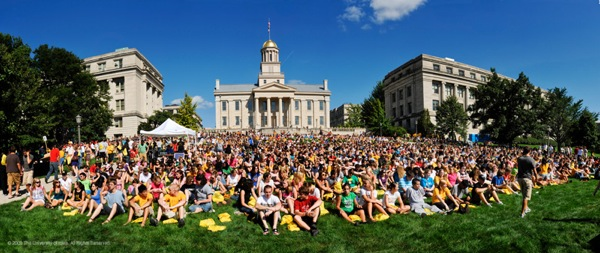
\includegraphics[width=0.6\columnwidth]{fig1}
    \label{fig:1}
\end{figure}


  %\section{heading 1: my chapter 1}

Heading 1 is the style you should use for the following headings in your thesis: List of Tables, List of Figures (List of Abbreviations, Schemes, and so on), Chapter titles, References, and Appendix titles. If you are writing in APA style, note that the titles formatted as Heading 1 do not count as an APA heading.  

I want to cite something here \parencite{zuo2019standing}. I want to want to try cite~\textcite{zuo2019standing} with in-line style.

\subsection{heading 2: Use for Your broadest Subheading Level, Centered, Bold, Title Case}

Heading 2 is the first major subheading style. If you are writing in APA style, this heading corresponds to a Level 1 APA heading.  

\subsubsection{heading 3: Use for Your Next Heading Level, Left-aligned, Bold, Title Case}

Heading 3 is the second major subheading style. If you are writing in APA style, this heading corresponds to a Level 2 APA heading. 

\paragraph{Heading 4: This Heading is Left-aligned, Boldface Italics, Title Case}
This is an additional heading level, should your thesis require this level of specificity.

Let me add a figure here~\cref{fig:1}:
\begin{figure}[h]
    \centering
    \captionsetup{width=0.6\linewidth} %% change width to adjust the caption alignment
    \caption{Old capital museum}
    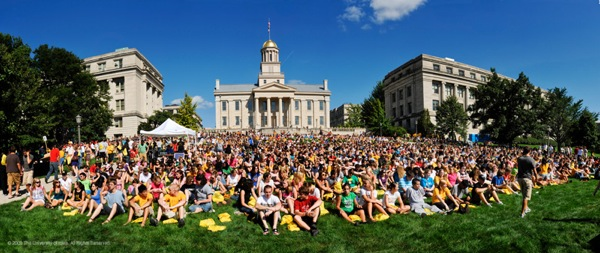
\includegraphics[width=0.6\columnwidth]{fig1}
    \label{fig:1}
\end{figure}

%\section{my chapter 2}

Lorem ipsum dolor sit amet, consectetuer adipiscing elit.  Ut purus elit, vestibulum ut, placeratac,  adipiscing vitae,  felis.   Curabitur dictum gravida mauris.  

Nam arcu libero,  nonummy eget,consectetuer id, vulputate a, magna. Donec vehicula augue eu neque. Pellentesque habitant morbitristique senectus et netus et malesuada fames ac turpis egestas. Mauris ut leo. Cras viverra metusrhoncus sem.  Nulla et lectus vestibulum urna fringilla ultrices. 

I want to cite something here \parencite{fennell2018predicting}. I want to want to try cite~\textcite{zuo2019standing} with in-line style.
Add this table here:

\begin{table}[ht]
    \centering
    \captionsetup{width=0.8\linewidth} %% change width to adjust the caption alignment
    \caption{Sample table}
    \begin{tabular}{cccccc}
         \hline
         \textbf{Column 1} & \textbf{Column}  & \textbf{Column 3} & \textbf{Column 4} & \textbf{Column 5} & \textbf{Column 6}\\
         \hline
         \textbf{Row 1} & 12.34 & 12.34 & 12.34 & 12.34 & 12.34 \\
         \hline
         \textbf{Row 2} & 12.34 & 12.34 & 12.34 & 12.34 & 12.34 \\
         \hline
    \end{tabular}
    \label{table:table1}
\end{table}

Lorem ipsum dolor sit amet, consectetuer adipiscing elit.  Ut purus elit, vestibulum ut, placeratac,  adipiscing vitae,  felis.   Curabitur dictum gravida mauris.  
Nam arcu libero,  nonummy eget,consectetuer id, vulputate a, magna. Donec vehicula augue eu neque. Pellentesque habitant morbitristique senectus et netus et malesuada fames ac turpis egestas. Mauris ut leo. Cras viverra metusrhoncus sem.  Nulla et lectus vestibulum urna fringilla ultrices~\cref{table:table1}. 


%\section{my chapter 3}

Lorem ipsum dolor sit amet, consectetuer adipiscing elit.  Ut purus elit, vestibulum ut, placeratac,  adipiscing vitae,  felis.   Curabitur dictum gravida mauris.  

Nam arcu libero,  nonummy eget,consectetuer id, vulputate a, magna. Donec vehicula augue eu neque. Pellentesque habitant morbitristique senectus et netus et malesuada fames ac turpis egestas. Mauris ut leo. Cras viverra metusrhoncus sem.  Nulla et lectus vestibulum urna fringilla ultrices. \textcite{zuo2017state}

Lorem ipsum dolor sit amet, consectetuer adipiscing elit.  Ut purus elit, vestibulum ut, placeratac,  adipiscing vitae,  felis.   Curabitur dictum gravida mauris.  
Nam arcu libero,  nonummy eget,consectetuer id, vulputate a, magna. Donec vehicula augue eu neque. Pellentesque habitant morbitristique senectus et netus et malesuada fames ac turpis egestas. Mauris ut leo. Cras viverra metusrhoncus sem.  Nulla et lectus vestibulum urna fringilla ultrices. 

Let me add another figure here:

\begin{figure}[h]
    \centering
    \captionsetup{width=0.7\linewidth} %% change width to adjust the caption alignment
    \caption{Kinnick stadium}
    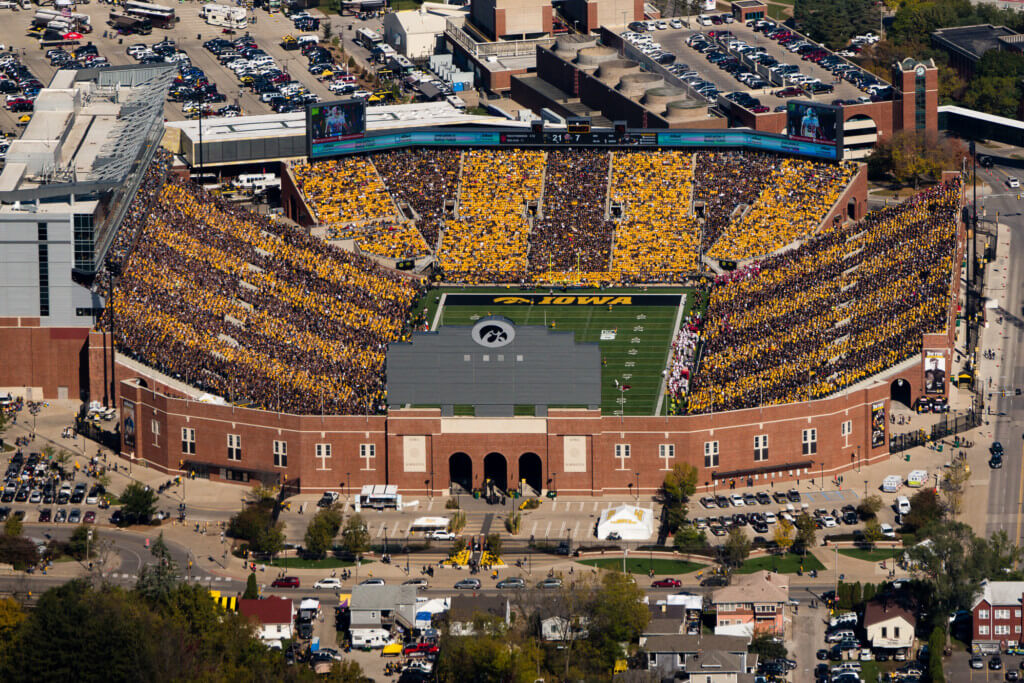
\includegraphics[width=0.7\columnwidth]{fig2}
    \label{fig:2}
\end{figure}

\subsection{heading 2: Use for Your broadest Subheading Level, Centered, Bold, Title Case}

Lorem ipsum dolor sit amet, consectetuer adipiscing elit.  Ut purus elit, vestibulum ut, placeratac,  adipiscing vitae,  felis.   Curabitur dictum gravida mauris~(\cref{fig:2}).  
Nam arcu libero,  nonummy eget,consectetuer id, vulputate a, magna. Donec vehicula augue eu neque. Pellentesque habitant morbitristique senectus et netus et malesuada fames ac turpis egestas. Mauris ut leo. Cras viverra metusrhoncus sem.  Nulla et lectus vestibulum urna fringilla ultrices. 

%% main contents %%

%% ref %%
\clearpage
%\section{references}
%\printbibliography[heading=none]
\bibliographystyle{unsrt}
\bibliography{ref.bib}
\nocite{*}
%% ref %%

%% appendix %%
%\appendix
%\newcommand{\hbAppendixPrefix}{A}
\renewcommand{\thefigure}{\hbAppendixPrefix.\arabic{figure}}
\setcounter{figure}{0}
\renewcommand{\thetable}{\hbAppendixPrefix.\arabic{table}} 
\setcounter{table}{0}

\let\svaddcontentsline\addcontentsline
\renewcommand\addcontentsline[3]{%
      \ifthenelse{\equal{#1}{lof}}{}%
        {\ifthenelse{\equal{#1}{lot}}{}{\svaddcontentsline{#1}{#2}{#3}}}}

\section{APPENDIX \hbAppendixPrefix: Numeric data}

The Appendix (A, B, and so on) heading is formatted as a Heading 1. Note that if you include only one Appendix, you do not need to assign it a letter. 

Make a table in Appendix A:
\begin{table}[ht]
    \centering
    \captionsetup{width=0.8\linewidth} %% change width to adjust the caption alignment
    \caption{Sample table}
    \begin{tabular}{cccccc}
         \hline
         \textbf{Column 1} & \textbf{Column}  & \textbf{Column 3} & \textbf{Column 4} & \textbf{Column 5} & \textbf{Column 6}\\
         \hline
         \textbf{Row 1} & 12.34 & 12.34 & 12.34 & 12.34 & 12.34 \\
         \hline
         \textbf{Row 2} & 12.34 & 12.34 & 12.34 & 12.34 & 12.34 \\
         \hline
    \end{tabular}
    \label{table:tableA1}
\end{table}

And I am going to ref this table~\cref{table:tableA1}.
Lorem ipsum dolor sit amet, consectetuer adipiscing elit.  Ut purus elit, vestibulum ut, placeratac,  adipiscing vitae,  felis.   Curabitur dictum gravida mauris.  
Lorem ipsum dolor sit amet, consectetuer adipiscing elit.  Ut purus elit, vestibulum ut, placeratac,  adipiscing vitae,  felis.   Curabitur dictum gravida mauris.  
Lorem ipsum dolor sit amet, consectetuer adipiscing elit.  Ut purus elit, vestibulum ut, placeratac,  adipiscing vitae,  felis.   Curabitur dictum gravida mauris.  
Lorem ipsum dolor sit amet, consectetuer adipiscing elit.  Ut purus elit, vestibulum ut, placeratac,  adipiscing vitae,  felis.   Curabitur dictum gravida mauris.  
Lorem ipsum dolor sit amet, consectetuer adipiscing elit.  Ut purus elit, vestibulum ut, placeratac,  adipiscing vitae,  felis.   Curabitur dictum gravida mauris.  

%\renewcommand{\hbAppendixPrefix}{B}
\renewcommand{\thefigure}{\hbAppendixPrefix.\arabic{figure}}
\setcounter{figure}{0}
\renewcommand{\thetable}{\hbAppendixPrefix.\arabic{table}} 
\setcounter{table}{0}

\section{APPENDIX \hbAppendixPrefix: Image data}

Lorem ipsum dolor sit amet, consectetuer adipiscing elit.  Ut purus elit, vestibulum ut, placeratac,  adipiscing vitae,  felis.   Curabitur dictum gravida mauris.
Let me add a figure here~\cref{fig:B1}:

\begin{figure}[h]
    \centering
    \captionsetup{width=0.7\linewidth} %% change width to adjust the caption alignment
    \caption{Old capital museum}
    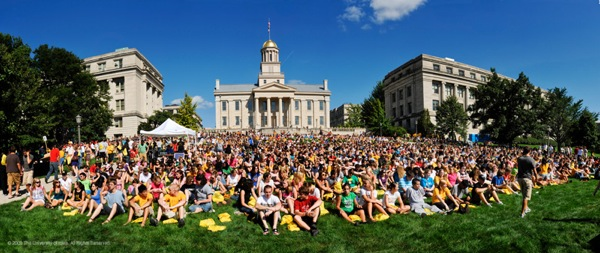
\includegraphics[width=0.7\columnwidth]{fig1}
    \label{fig:B1}
\end{figure}

%% appendix %%


%\end{doublespace}


\end{document}
